\label{chapter:binary}
\label{binarychapter}

In this chapter we will review two current simplified binary PFC models.
The first is the original binary PFC model of Elder \textit{et al.}
\cite{ELDER07} and the second is the binary structural PFC model  
model of Greenwood \textit{et al.} \cite{GREENWOOD11_BINARY} 
--coined the binary XPFC model. We begin 
by establishing background shared by  all binary PFC models and move on 
to summarize and review each.

We begin with a multicomponent variant of the approximate
free energy functional established in Chapter \ref{chapter:cdft_intro},
%
\begin{align}
    \label{binary_cdft_free_energy}
    \beta\F[\A, \B] &= \sum_{i=A, B} \int \mathrm{d}r 
        \,\rho_i(r) \ln\l(\f{\rho_i(r)}{\rho_i^0}\r) 
        - (1 - \beta\mu_i^0)\Delta\rho_i(r)\\
    &- \f{1}{2} \sum_{i,j=A, B} \Delta\rho_i(r) \ast C^{(2)}_{ij}(r, r^\prime) 
        \ast \Delta\rho_j(r^\prime). \nonumber
\end{align}
%
It is convenient to change variables to a dimensionless total density, $n(r)$
and local concentration, $c(r)$,
%
\begin{gather}
    n(r) = \f{\Delta \rho}{\rho_0} = \f{\Delta\A + \Delta\B}{\A^0 + \B^0} \\
    c(r) = \f{\B}{\rho} = \f{\B}{\A + \B}.
\end{gather}
%
Scaling out a factor of the total reference density, $\rho_0$ we can break the
free energy functional in these new variables into three parts,
%
\begin{equation}
    \label{binary_total_free_energy}
    \f{\beta\F[n, c]}{\rho_0} = \f{\beta\F_{id}[n]}{\rho_0} 
        + \f{\beta\F_{mix}[n, c]}{\rho_0}
        + \f{\beta\F_{ex}[n, c]}{\rho_0},
\end{equation}
%
where,
%
\begin{gather}
    \label{binary_ideal}
    \f{\beta\F_{id}[n]}{\rho_0} =
        \int \mathrm{d}r \,\l\lbrace (n(r) + 1)\ln(n(r) + 1) 
        - (1 - \beta\mu^0)n(r) \r\rbrace \\
    \label{binary_mixing}
    \f{\beta\F_{mix}[n, c]}{\rho_0} =
        \int \mathrm{d}r \,\l\lbrace (n(r) + 1)\l( 
            c\ln\l(\f{c}{c_0}\r) + (1-c)\ln\l(\f{1-c}{1-c_0}\r) \r)\r\rbrace, 
\end{gather}
%
\nc{where we have introduced $\mu^0=\mu_1^0+\mu_2^0+\cdots$ as the total chemical potential of the reference
mixture, and $c_0 = \B^0 / \rho_0$ as the reference concentration.} Assuming that the local concentration $c(r)$ varies over much longer length scales than the local density $n(r)$, the excess free energy term becomes  
%
\begin{align}
    \label{binary_excess}
    \f{\beta\F_{ex}[n, c]}{\rho_0}
        = &-\f{1}{2} n(r) \ast \l[ 
            C_{nn}(r, r^\prime) \ast n(r^\prime) 
          + C_{nc}(r, r^\prime) \ast \Delta c(r^\prime)\r] \\
        &-\f{1}{2} \Delta c(r) \ast \l[
            C_{cn}(r, r^\prime) \ast n(r^\prime) 
          + C_{cc}(r, r^\prime) \ast \Delta c(r^\prime)\r], \nonumber
\end{align}
%
where we have introduced  and $\Delta c(r) = c(r) - c_0$ as the deviation of the 
concentration from the reference.  The $n-c$ pair correlation introduced in the 
excess free energy are,
%
\begin{align}
    C_{nn} &= \rho_0\l(c^2 C_{BB} + (1 - c)^2C_{AA} + 2c(1-c)C_{AB}\r) \label{orig_nnC}\\
    C_{nc} &= \rho_0\l(c C_{BB} - (1 - c) C_{AA} + (1 - 2c)C_{AB}\r) \\
    C_{cn} &= C_{nc} \\
    C_{cc} &= \rho_0\l(C_{BB} + C_{AA} - 2 C_{AB}\r)
\end{align}
%
Explicit \nc{derivations of these terms} can be found in Appendix \ref{appendix:binary_corr}.
Differences in the various simplified binary PFC theories stem from differing
approximations of the terms in the free energy stated in equations 
\ref{binary_ideal}, \ref{binary_mixing} and \ref{binary_excess}.

%%%%%%%%%%%%%%%%%%%%%%%%%%%%%%%%%%%%%%%%%%%%%%%%%%%%%
\section{Original Binary Phase Field Crystal Model} %
%%%%%%%%%%%%%%%%%%%%%%%%%%%%%%%%%%%%%%%%%%%%%%%%%%%%%

In the original simplified binary PFC theory, all terms in the free energy are
expanded about $n(r) = 0$ and $c(r) = c_0$ (ie., about their reference states).
For the ideal free energy this results in a polynomial truncated to fourth
order,
%
\begin{equation}
    \label{ideal_expansion}
    \f{\beta\F_{id}[n]}{\rho_0} = \integrate{r}
    \l\lbrace \f{n(r)^2}{2} - \eta\f{n(r)^3}{6} + \chi\f{n(r)^4}{12} \r\rbrace.
\end{equation}
%
The linear term in the expansion is dropped by redefining $n$ about its average
and we have added the fitting parameters $\eta$ and $\chi$ to fit the free
energy away from the reference parameters. If we assume for simplicity of
demonstration $c_0 = 1/2$, the free energy of mixing becomes a simple fourth
order polynomial as well,
%
\begin{equation}
    \f{\beta\F_{mix}[n, c]}{\rho_0} = \integrate{r} \l\lbrace
       2\Delta c(r)^2 + \f{4\Delta c(r)^4}{3}
    \r\rbrace.
\end{equation}
%
Linear couplings to $n(r)$ are dropped by assuming, as we already have, that
the concentration field varies on a much longer length scale than the total
density and noting that the total density is defined about its average. This
argument can also be applied to the linear couplings to $n(r)$ in the excess free
energy term, which then leaves only the $C_{nn}$ and $C_{cc}$ terms. Finally, these
two terms are approximated with a gradient expansion of the form,
%
\begin{gather}
    C_{nn}(r, r^\prime) = \d(r - r^\prime)\l(
        C_0 + C_2 \nabla^2 + C_4 \nabla^4 + \dots\r), \\
    C_{cc}(r, r^\prime) = \d(r - r^\prime)\l(
        \epsilon + W_c \nabla^2 + \dots\r).
\end{gather}
%
\nb{Note that as actual functions, the delta functions should formally be to the right with the gradients acting on them. They are removed by integrating the double integrals in the excess terms by parts. This makes them perators, which is fine} The expansion parameters, $C_0, C_2,$ and $C_4$ are all dependent on
temperature and concentration. We are required to expand $C_{nn}$ to fourth
order because, as noted in chapter \ref{chapter:cdft_of_freezing}, the peak of
the direct correlation function in Fourier space is the driving force for
solidification.  The concentration field is correlated over a longer length
scale implying that only the short wavevectors are important in $C_{cc}$ so we
can expand just to quadratic order, \nc{effectively treating $c$ as in the 
traditional Cahn-Hilliard theory}.

Gathering terms, the resulting free energy functional for the original simplified
binary PFC model\footnote{The orignal simplified binary PFC model was
expressed using slightly different variables. We expand in $\Delta c(r)$ here to 
facilitate comparison with other theories} is,
%
\begin{align}
    \f{\beta\F[n, c]}{\rho_0} &= \integrate{r} \l\lbrace 
        \f{1}{2} n(r) \l( 1 - C_0 - C_2 \nabla^2 - C_4\nabla^4 \r) n(r)
      - \eta\f{n(r)^3}{6} + \chi\f{n(r)^4}{12} \r\rbrace \\
    &+ \integrate{r} \l\lbrace
        \f{1}{2} \Delta c(r) \l( 4 - \epsilon - W_c\nabla^2 \r) \Delta c(r) 
      + \f{4 \Delta c(r)^4}{3} \r\rbrace. \nonumber
\end{align}
%

The strength of the original simplified binary PFC model is that is retains
most of the important physics of binary alloys in a very reduced theory. For
instance, the simplified model is capable of describing the equilibrium phase
diagrams of both eutectic alloys and materials with a solid state spinodal /
liquid minimum.  Supplied with a diffusive equation of motion, the simplified
model can model an impressive diversity of dynamic phenomena including eutectic
growth \cite{ELDER07}, solute segregation \cite{STOLLE14}, dendritic growth
\cite{ELDER07}, epitaxial growth \cite{ELDER10_NANOISLAND, LU16} and crack
formation \cite{HU17}.

The major limitation of the original simplified model is that the gradient
expansion of the density-density correlation function gives only a crude
control over the crystal structures that can be formed. In fact, as this theory only
controls a single peak in Fourier space it can only solidify into the BCC
phase. As noted in chapter \ref{chapter:cdft_of_freezing}, the ability to
solidify into an arbitrary structure demands control of the
density-density correlation function at all reciprocal lattice vectors.

A second limitation of the original simplified model is that it is local in
concentration. This means that realistic phase diagrams from 0 to 100\%
concentration cannot be produced, only local phase diagrams around the
reference concentration
%%%
\nc{\footnote{Indeed, the original model "concentration" was in fact a density difference, not  true concentration.}. }
%%%%
To construct \nc{experimentally relevant} phase diagrams, we require
the entire free energy of mixing term in equation \ref{binary_mixing}. \nc{It 
is important to mention that global phase diagram couched in terms of 
the variable $c$ is important for sharing binary PFC results with the wider 
material science community, and establishing a shared language. }

%%%%%%%%%%%%%%%%%%%%%%%%%%%%%%%%%%%%%%%%%%%%%%%%%%%%%%%
\section{Original Binary Structural Phase Field Crystal  Model} %
%%%%%%%%%%%%%%%%%%%%%%%%%%%%%%%%%%%%%%%%%%%%%%%%%%%%%%%

The binary structural phase field crystal theory (XPFC) seeks to remedy the two
short comings of the original simplified model. That is, it seeks to construct
realistic phase diagrams for binary systems and seeks to reproduce a variety 
of crystal lattice structure. We'll begin with a derivation of the theory and
compare with the original model.

First, the ideal free energy is expanded in precisely the same manner resulting
in the same fourth order polynomial,
%
\begin{equation}
    \f{\beta\Delta\F_{id}[n]}{\rho_0} = \integrate{r}
        \l\lbrace \f{n(r)^2}{2} - \eta \f{n(r)^3}{6} + \chi\f{n(r)^4}{12}
        \r\rbrace. \tag{\ref{ideal_expansion} revisited}
\end{equation}
%
The free energy of mixing is left unexpanded but an overall scale $\omega$ is
added to fit the mixing term away from the reference concentration,
%
\begin{equation}
    \f{\beta\F_{mix}[n, c]}{\rho_0} =
        \integrate{r} \l\lbrace \omega (n(r) + 1)\l( 
            c\ln\l(\f{c}{c_0}\r) + (1-c)\ln\l(\f{1-c}{1-c_0}\r) \r)\r\rbrace. 
\end{equation}
%
This unexpanded free energy of mixing will lead to more accurate global phase
diagrams. The excess free energy is approximated using similar assumptions as
in the original model (linear couplings are dropped), but the density-density
correlation function, $C_{nn}$, is not expanded. Instead, Greenwood \textit{et al} all
assumed that the $k=0$ mode of the concentration-concentration correlation
function was zero leaving only the quadratic term in the expansion,
%
\begin{equation}
    C_{cc}(r, r^\prime) = \d(r - r^\prime)W_c \nabla^2.
\end{equation}
%
Grouping terms together, the complete free energy functional for the binary XPFC
model is,
%
\begin{align}
    \f{\beta\Delta\F[n, c]}{\rho_0} &= \integrate{r} \l\lbrace
        \f{1}{2} n(r) \l(1 - C_{nn}(r, r^\prime)\r) \ast n(r^\prime)
        - \eta \f{n^3}{6} + \chi \f{n^4}{12} \r\rbrace \\
        &+ \integrate{r}\l\lbrace
            \f{W_c}{2}\l\vert \nabla c(r) \r\vert^2 + \omega f_{mix}(r)
            \r\rbrace. \nonumber
\end{align}
%
Where $f_{mix}(r)$ is the local free energy density of mixing,
%
\begin{equation}
    f_{mix}(r) = \l(n(r) + 1\r)\l( 
            c(r)\ln\l(\f{c(r)}{c_0}\r) + (1-c(r))\ln\l(\f{1-c(r)}{1-c_0}\r) \r).
\end{equation}
%

The density-density correlation function, $C_{nn}$, is left unexpanded in 
Fourier space but assumed to have a specific phenomenological form,
%
\begin{equation}
    \label{eq:xpfc_corr}
    C_{nn} = \zeta_A(c) C_{AA}(r, r^\prime) 
           + \zeta_B(c) C_{BB}(r, r^\prime),
\end{equation}
%
where $\zeta_A(c)$ and $\zeta_B(c)$ are interpolation functions, assigned the forms
%
\begin{gather}
    \zeta_A(c) = 1 - 3c^2 + 2c^3 \\
    \zeta_B(c) = \zeta_A(1 - c).
\end{gather}
%
by Greenwood \textit{et al.}

The remaining elemental correlation functions $C_{AA}$ and $C_{BB}$ are modelled
using the general XPFC model for correlation functions, which we describe
subsequently.

%%%%%%%%%%%%%%%%%%%%%%%%%%%%%%%%%%%%%%%%%%%%%%
\subsection{XPFC Correlation Functions} %
%%%%%%%%%%%%%%%%%%%%%%%%%%%%%%%%%%%%%%%%%%%%%%

The key insight made by the XPFC model is that the density-density
correlation function can be modelled in such a way as to control the crystal
lattice structure formed under solidification and to target different structures at
different concentrations, \nc{and temperatures}.  Originally delineated for pure systems, the XPFC
method for constructing correlation functions is strongly influenced by the
methods developed by Ramakrishnan. In particular this means that we need a
model correlation function that controls the values specifically at the
reciprocal lattice vector positions. We can achieve this with Gaussian peaks
centred at the reciprocal lattice vector positions,
%
\begin{equation}
    \tilde{C}(k) = \sum_{\alpha} e^{\f{T}{T_\alpha^0}}
        e^{ - \f{(k - k_\alpha)^2}{2\sigma_\alpha^2}}
        \label{XPFC_C2}
\end{equation}
%
Where, as in chapter \ref{chapter:cdft_of_freezing}, the index $\alpha$ runs
over families of point group symmetry-equivalent reciprocal lattice vectors, $k_\alpha$
is the length of the reciprocal lattice vectors in $\alpha$ and $\sigma_\alpha$
is the width of the peak. Temperature dependence of the correlation peaks in the 
is achieved through the prefactors $e^{T /
T_\alpha^0}$ give the correct temperature scaling of the amplitudes close to
the melting point \footnote{The original XPFC works used a phenomenological
prefactor $e^{\sigma^2 / C_i}$, where $\sigma$ was considered a model temperature 
parameter and $C_i$ a constant. The present choice used in this thesis is inspired by
harmonic analysis in the solid phase and the Debye-Waller factor.} as discussed
by \cite{ALSTER17}. \nb{what is $T_\alpha^0$?}

The primary advantages of the XPFC model are two fold: they produce realistic phase 
diagrams and they model a variety of crystalline lattices. While the former is relatively
cosmetic the latter allows for the examination of genuinely novel systems in
comparison with the original simplified model. For example, the binary XPFC
model has been used to study peritectic systems \cite{GREENWOOD11_BINARY}, 
ordered crystals \cite{ALSTER17}, dislocation-assisted solute clustering and precipitation 
\cite{FALLAH12, FALLAH13} and solute drag \cite{GREENWOOD12}. \nc{It is noteworthy, 
that the above works on clustering was validated experimentally in binary and ternary alloys.}

\begin{figure}
    \centering
    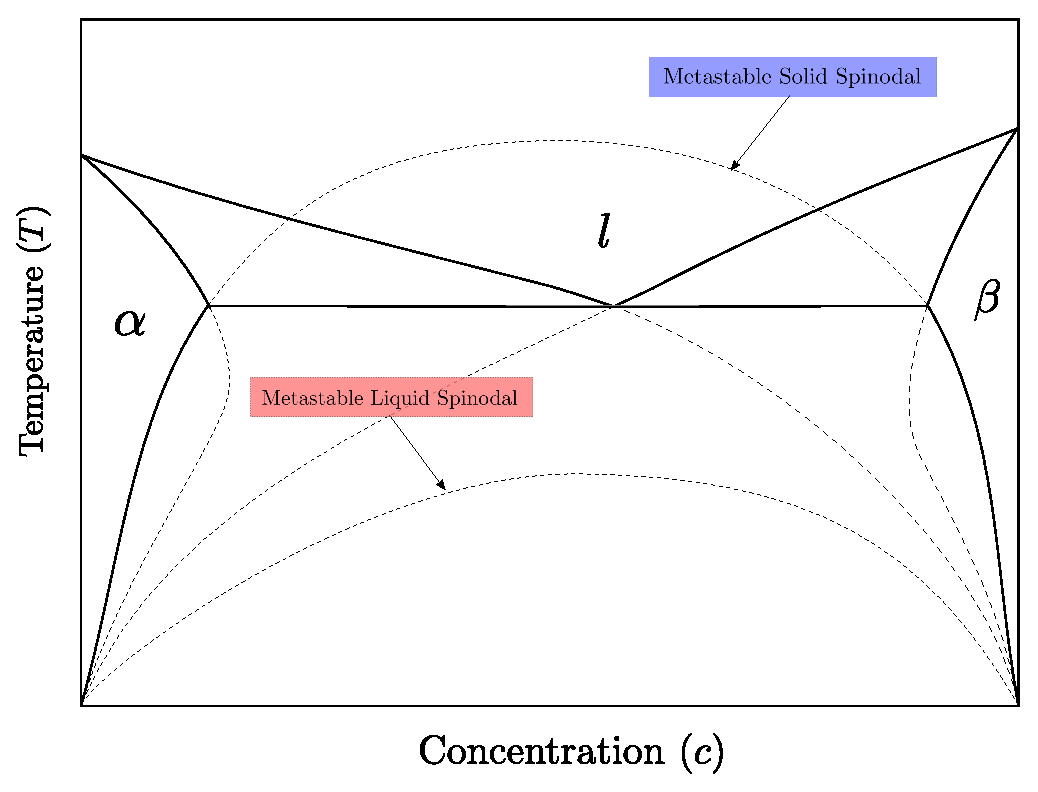
\includegraphics[scale=0.7]{eutectic-drawing}
    \caption[Eutectic Phase Diagram with Metastable Projections]{
        \label{fig:eutectic_drawing} Eutectic phase diagram with metastable
        projections. Stable coexistance lines are rendered solid whereas 
        metastable projections are dashed. \nb{should you also point to the solid-liquid metastable projections?}
    }
\end{figure}

Unfortunately, by assuming that the $k=0$ mode of the
concentration-concentration correlation function is zero, the XPFC model
restricts its free energy of mixing to an ideal model of mixing. This model
of mixing includes only entropic contributions to the free energy. \nc{In the solid state, 
this means} that the sole driving force for phase separation is elastic energy as the enthapy
of mixing is always zero. This \nc{is also precludes the} modelling a variety of binary
alloy systems, for instance both monotectic and syntectic systems cannot be
modelled without a negative enthalpy of mixing. More subtly, \nc{in the present XPFC 
alloy model, even eutectic systems} have a negative heat of mixing deep 
below the eutectic point as the metastable liquid has a spinodal. This 
phenomena is shown schematically in figure \ref{fig:eutectic_drawing}, 
where the metastable projections, including solid and liquid spinodals, 
are drawn on a hypothetical eutectic phase diagram. Problems such as 
the stability of nanocrystalline binary alloys require an examination that 
balances elastic energies and bulk mixing free energy \cite{MURDOCH13}.

A second disadvantage of the \nc{present} XPFC model is that the phenomenological form for
the correlation function as seen in equation \ref{eq:xpfc_corr} implicitly
assumes that there are well defined structures at $c=0$ and $c=1$. This works
well for modelling eutectic systems for example, but does not work very well
when we expect a solid phase at intermediate concentration. \nc{This thesis will offer 
improvements} to both of these shortcomings in the following chapter.

